\documentclass[11pt,a4paper]{article}

\usepackage{amsmath}
\usepackage{graphicx}
\usepackage{epstopdf}

\title{AMTH250 \\ Assignment 5}

\author{Mark Villar}

\begin{document}

\maketitle

\subsubsection*{Question 1} 
\begin{enumerate}
	\item[(a)] Solution to the system of linear equations (to 2 decimal places):
	\begin{center}
		\begin{tabular}{|c|c|}
		\hline
		Parameter &Estimate \\
		\hline
			$x_1$ &-28.28 \\
			$x_2$ &20.00 \\
			$x_3$ &10.00 \\
			$x_4$ &-30.00 \\
			$x_5$ &14.14 \\
			$x_6$ &20.00 \\
			$x_7$ &0.00 \\
			$x_8$ &-30.00 \\
			$x_9$ &7.07 \\
			$x_{10}$ &25.00 \\
			$x_{11}$ &20.00 \\
			$x_{12}$ &-35.36 \\
			$x_{13}$ &25.00 \\
		\hline
		\end{tabular}
	\end{center}
	The estimated relative error is $2.312\times10^{-15}$.
		
	\item[(b)] The actual relative error is $1.382\times10^{-16}$. We have overestimated the error by a factor of 16.729.

	\item[(c)] The \emph{real} eigenvalues of the matrix are $\lambda_1=-1.2728, \ \lambda_2=0.72297$ and $\lambda_3=0.51150$. Their corresponding eigenvectors are given below. 
	\pagebreak
		\begin{align*}
		v_1=
		\begin{bmatrix}
			 0.270745 \\ 
			0.105756 \\
			-0.134606 \\
			-0.282125 \\
			0.427441 \\
			0.450357 \\
			-0.573209 \\
			0.261916 \\
			-0.088249 \\
			0.085430 \\
			-0.108734 \\
			0.086436 \\
			-0.026892 
		\end{bmatrix} 
		\quad v_2=
		\begin{bmatrix}
			 -0.217392 \\
			0.398094 \\
			0.287809 \\
			-0.132159 \\ 
			-0.324755 \\
			0.555261 \\
			0.401436 \\
			0.102629 \\
			-0.138030 \\
			0.133001 \\
			0.096156 \\
			-0.091204 \\
			0.232792
		\end{bmatrix}
		\quad v_3=
		\begin{bmatrix}
			 -0.1703240 \\
			0.3917440 \\
			0.2003763 \\
			-0.0946017 \\
			-0.1814827 \\
			0.4788643 \\
			0.2449382 \\
			-0.0017736 \\
			-0.1661952 \\
			0.3427691 \\
			0.1753257 \\
			-0.2955285 \\
			0.4277776
		\end{bmatrix}
	\end{align*}
\end{enumerate}

\subsubsection*{Question 2}
\begin{enumerate}
	\item[(a)] Graph of $\log_{10}$ of the condition number of $\mathbf{H}_n$ as a function of $n$ for $n=1, \ldots , 30$.
	\begin{center}
		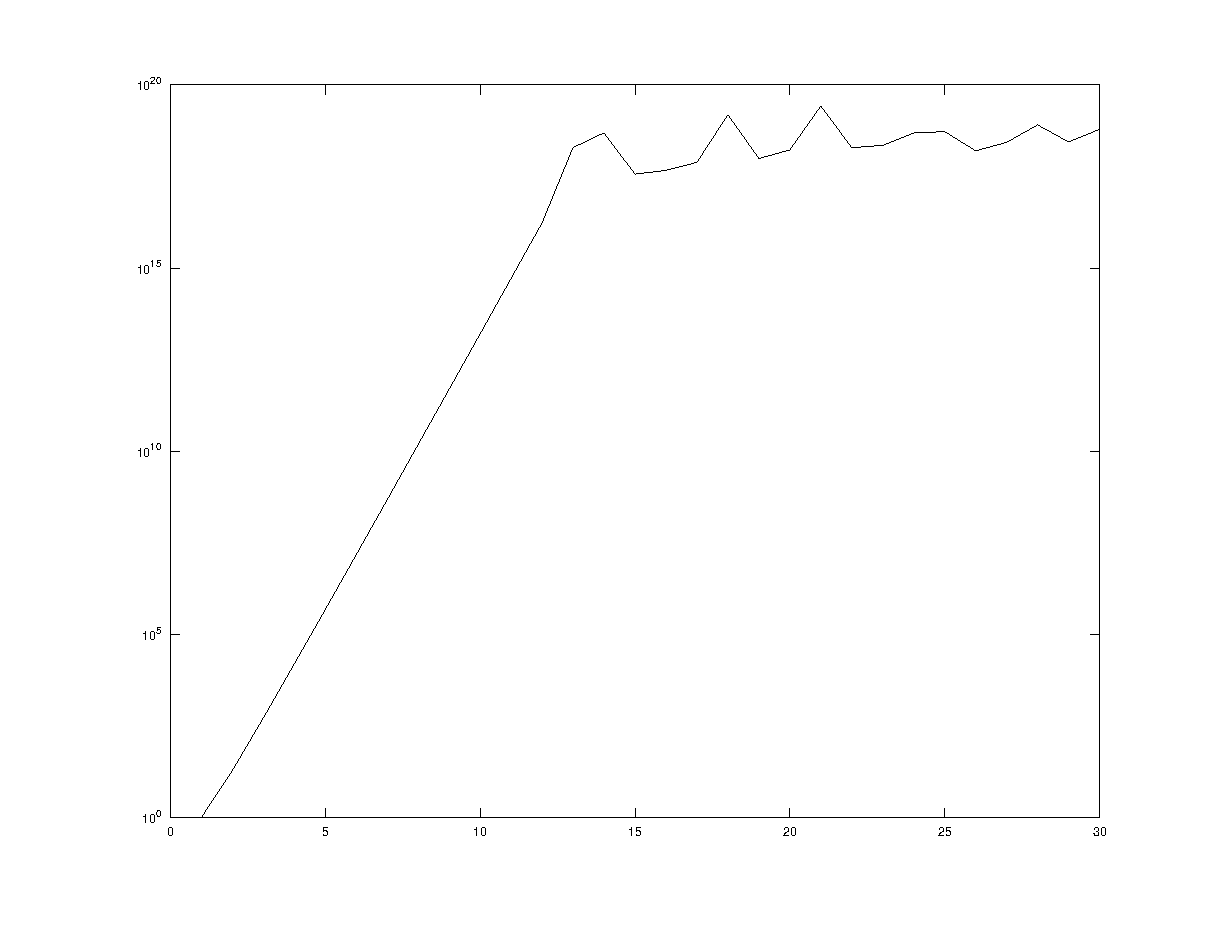
\includegraphics[width=1.1\textwidth]{chilb.eps}
	\end{center}
	\item[(b)] The condition number is an increasing function of $n$ for $n<14$. For $n \ge 14$, the condition number no longer appears to depend on $n$.
	\item[(c)] $n$ can be as large as 8 to obtain a relative error less than $10^{-4}$. When $n=9$, the relative error is $1.0950 \times 10^{-4}$, which is slightly greater than $10^{-4}$.
	\item[(d)] Minimum and maximum eigenvalues of $\mathbf{H}_n$ for $n=1, \ldots , 30$.	
	\begin{center}
		\begin{tabular}{|c|c|c|}
			\hline
			$n$ &Minimum &Maximum \\
			\hline
			1 &1.0000 &1.0000 \\
			2 &$6.5741 \times 10^{-2}$ &1.2676 \\ 
			3 &$2.6873 \times 10^{-3}$ &1.4083 \\
			4 &$9.6702 \times 10^{-5}$ &1.5002 \\
			5 &$3.2879 \times 10^{-6}$ &1.5671 \\
			6 &$1.0828 \times 10^{-7}$ &1.6189 \\
			7 &$3.4939 \times 10^{-9}$ &1.6609 \\
			8 &$1.1115 \times 10^{-10}$ &1.6959 \\
			9 &$3.4997 \times 10^{-12}$ &1.7259 \\
			10 &$1.0930 \times 10^{-13}$ &1.7519 \\
			11 &$3.4304 \times 10^{-15}$ &1.7749 \\
			12 &$6.9144 \times 10^{-17}$ &1.7954 \\
			13 &$1.2865 \times 10^{-17}$ &1.8138 \\
			14 &$8.6284 \times 10^{-18}$ &1.8306 \\
			15 &$4.8009 \times 10^{-18}$ &1.8459 \\
			16 &$6.4139 \times 10^{-18}$ &1.8600 \\
			17 &$5.0873 \times 10^{-18}$ &1.8731 \\
			18 &$1.9835 \times 10^{-18}$ &1.8852  \\
			19 &$9.0863 \times 10^{-19}$ &1.8965 \\
			20 &$2.6251 \times 10^{-18}$ &1.9071 \\
			21 &$2.8938 \times 10^{-18}$ &1.9171 \\
			22 &$3.5883 \times 10^{-18}$ &1.9265 \\
			23 &$9.7868 \times 10^{-19}$ &1.9354 \\
			24 &$1.5220 \times 10^{-18}$ &1.9438 \\
			25 &$2.5270 \times 10^{-19}$ &1.9518 \\
			26 &$5.5925 \times 10^{-19}$ &1.9594 \\
			27 &$1.6187 \times 10^{-18}$ &1.9666 \\
			28 &$1.2497 \times 10^{-18}$ &1.9735  \\
			29 &$1.2939 \times 10^{-18}$ &1.9801 \\
			30 &$5.4938 \times 10^{-19}$ &1.9865 \\
			\hline
		\end{tabular}
	\end{center}
	
	\begin{center}
		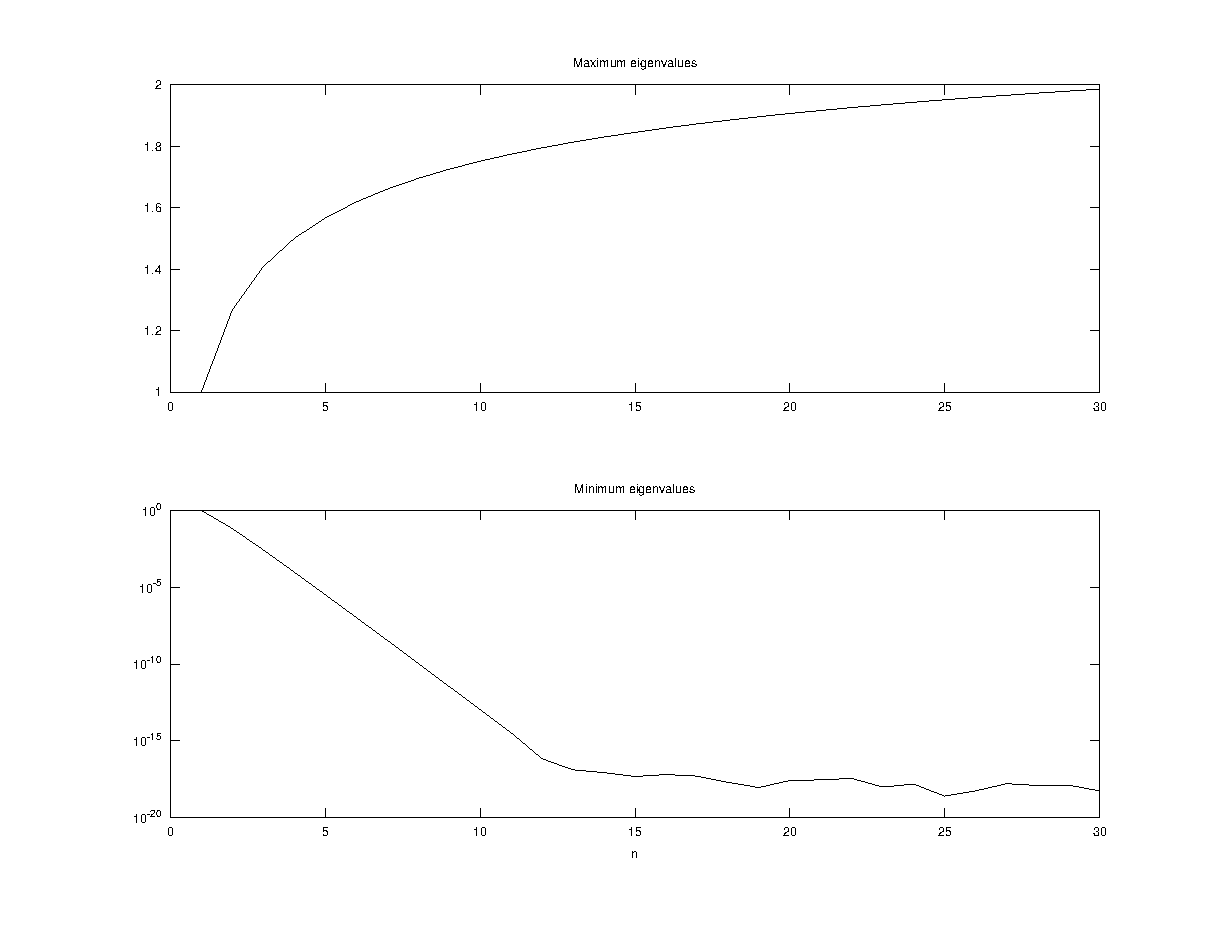
\includegraphics[width=1.05\textwidth]{minmax.eps}
	\end{center}
	
	Maximum eigenvalues as a function of $n$ increases at a decreasing rate and appears to approach a limit of 2.  For $n \le 12$, minimum eigenvalues are a decreasing function of $n$, otherwise the dependence no longer seems to exist.
	
	\item[(e)] The computed eigenvalues of $\mathbf{H}_n$ are real and positive for $n \le 12$.
	
	\item[(f)] 
	\begin{verbatim}
		1.0000e+000  1.0000e+000  1.0000e+000
		1.9281e+001  1.2676e+000  6.5741e-002
		5.2406e+002  1.4083e+000  2.6873e-003
		1.5514e+004  1.5002e+000  9.6702e-005
		4.7661e+005  1.5671e+000  3.2879e-006
		1.4951e+007  1.6189e+000  1.0828e-007
		4.7537e+008  1.6609e+000  3.4939e-009
		1.5258e+010  1.6959e+000  1.1115e-010
		4.9315e+011  1.7259e+000  3.4997e-012
		1.6025e+013  1.7519e+000  1.0930e-013
		5.2124e+014  1.7749e+000  3.4304e-015
		1.7033e+016  1.7954e+000  6.9144e-017
	\end{verbatim}
	The larger the condition number, the greater the difference between the minimum and maximum eigenvalues. Hence, our solution is more sensitive to numerical errors as $n$ increases.
	
	\item[(g)] Our answer to (e) suggests that the Octave results for (a) and (d) are reliable for $n \le 12$. However, if we look at the condition number in exponential notation $a \times 10^k$, the number of significant figures that should be believed is $15-k$ (as a rule of thumb). We see from (f) that $n \le 11$ is required to ensure $k<15$ and thereby, not all the result can be ignored and the rule of thumb is satisfied.
\end{enumerate}

\subsubsection*{Question 3}
To formulate the objective function we first determined the machine costs, summarised below.
\begin{center}
	\begin{tabular}{|c|c|}
		\hline
		Product &Machine Cost (\$) \\
		\hline
		A &4.65 \\
		B &4.50 \\
		C &5.00 \\
		D &4.80 \\
		E &1.95 \\
		\hline
	\end{tabular}
\end{center}
We then denote the number of units of each product by $x_i$ and maximise the following objective function
$$P=5.35x_A+4.5x_B+5x_C+4.7x_D+3.05x_E$$
subject to the following constraints
\begin{align*}
	&15x_A+8x_B+8x_C+12x_D+9x_E \le 4800 \\
	&8x_A+10x_B+12x_C+4x_D+4x_E \le 4800 \\
	&6x_A+9x_B+10x_C+12x_D \le 4800 \\
	&x_A, x_B, x_E \ge 0 \\
	&x_C \ge 20 \\
	&x_D \ge 30
\end{align*}
The optimal solution to this linear programming problem is given below, with a maximum profit of $\$2469$.
\begin{center}
	\begin{tabular}{|c|c|}
		\hline
		Product &Units \\
		\hline
		A &1 \\
		B &6 \\
		C &330 \\
		D &120 \\
		E &73 \\
		\hline
	\end{tabular}
\end{center}

\pagebreak

\textbf{Appendix}

\begin{enumerate}

\item
\begin{enumerate}
	
	\item
	\begin{verbatim}
		%solves a system the 13x13 system of linear equations 
		%and estimates the error
		
		k=sqrt(2)/2; %alpha

		a=zeros(13,13); %initialise matrix and rhs to zeros
		b=zeros(13,1);

		a(1,2)=1; %1st equation
		a(1,6)=-1;

		a(2,3)=1; %2nd equation
		b(2)=10;

		a(3,1)=k;
		a(3,4)=-1;
		a(3,5)=-k;

		a(4,1)=k;
		a(4,3)=1;
		a(4,5)=k;

		a(5,4)=1;
		a(5,8)=-1;

		a(6,7)=1;

		a(7,5)=k;
		a(7,6)=1;
		a(7,9)=-k
		a(7,10)=-1;

		a(8,5)=k;
		a(8,7)=1;
		a(8,9)=k;
		b(8)=15;

		a(9,10)=1;
		a(9,13)=-1;

		a(10,11)=1;
		b(10)=20;
		
		a(11,8)=1;
		a(11,9)=k;
		a(11,12)=-k;

		a(12,9)=k;
		a(12,11)=1;
		a(12,12)=k;

		a(13,12)=k;
		a(13,13)=1;

		x=a\b;
		esterr=cond(a)*eps;
		disp("Solution:"), disp(x)
		disp("Estimated error:"), disp(esterr)

	\end{verbatim}
		
	\item
	\begin{verbatim}
		%compares estimated and actual errors for the 13x13 system 
		%of linear equations
		
		x0=zeros(13,1);
		
		x0(1)=-20*sqrt(2);
		x0(2)=20;
		x0(3)=10;
		x0(4)=-30;
		x0(5)=10*sqrt(2);
		x0(6)=20;
		x0(7)=0;	
		x0(8)=-30;
		x0(9)=5*sqrt(2);
		x0(10)=25;
		x0(11)=20;
		x0(12)=-25*sqrt(2);
		x0(13)=25;

		err=norm(x-x0)/norm(x0);
		disp("Actual error:"), disp(err)
		disp("Ratio estimate/actual:"), disp(esterr/err)
	
	\end{verbatim}
	
	\pagebreak
	
	\item	
	\begin{verbatim}
		%computes the real eigenvalues of the matrix and their
		%corresponding eigenvectors
		
		eig(a)
		[V,D]=eig(a)
		
		k1=D(1,1)
		v1=V(:,1)

		k12=D(12,12)
		v12=V(:,12)

		k13=D(13,13)
		v13=V(:,13)
	\end{verbatim}
	
\end{enumerate}

\item
\begin{enumerate}
	\item
	\begin{verbatim}
		%graphs the ln of the condition number of the Hilbert matrix 
		%as a function of n
		chilb=zeros(30,1);
		for n=1:30
		chilb(n)=cond(hilb(n));
		end
		semilogy(chilb)
		print('chilb.eps','-deps')
	\end{verbatim}
	
	\item[(c)]
	\begin{verbatim}
		%computes the relative error in the solution for n=8,9
		chilb(8)*eps
		chilb(9)*eps
	\end{verbatim}
	
	\item[(d)]
	\begin{verbatim}
		%finds the minimum and maximum eigenvalues of the
		%Hilbert matrix for n=1,...,30
		maxeig = zeros(30,1);
		mineig = zeros(30,1);
		for n = 1:30
			eighilb = abs(eig(hilb(n)));
			maxeig(n) = max(eighilb);
			mineig(n) = min(eighilb);
		end
		subplot(2,1,1)
		plot(maxeig)
		title('Maximum eigenvalues')
		subplot(2,1,2)
		semilogy(mineig)
		title('Minimum eigenvalues')
		xlabel('n')
		print('maxeig.eps','-deps')
	\end{verbatim}
	
	\pagebreak
	
	\item[(e)]
	\begin{verbatim}
		t=1:1:12;
		comp=[chilb(t) maxeig(t) mineig(t)]
	\end{verbatim}
	
\end{enumerate}

\item
\begin{verbatim}
	%calculates the machine costs by multiplying the time on each
	%machine by the hourly rate of operating it
	time=[15 8 6; 8 10 9; 8 12 10; 12 4 12; 9 4 0];
	rate=[9;9;12];
	cost=ones(5,1);
	cost=1/60*time*rate
	
	%solves profit maximisation problem
	obj=[5.35 4.5 5 4.7 3.05]'
	cnstr=[15 8 8 12 9; 8 10 12 4 4; 6 9 10 12 0]
	rhs=[4800,4800,4800]
	lb=[0 0 20 30 0]'
	ub=[]
	ctype="UUU"
	vtype="IIIII"
	ptype=-1
	[x,opt]=glpk(obj,cnstr,rhs,lb,ub,ctype,vtype,ptype)
\end{verbatim}
	
\end{enumerate}

\end{document}